\documentclass{beamer}
\usepackage{moreverb} 
\usepackage{listings}
\usepackage{mflogo}
% imprimir
% \documentclass[handout]{beamer} 
% \usepackage{pgfpages}
% \pgfpagesuselayout{4 on 1}[a4paper,landscape,border shrink=5mm]

\mode<presentation> {
  \usetheme{Warsaw}
  \setbeamercovered{transparent}
}

\usebackgroundtemplate{
\includegraphics[width=\paperwidth]{format/libresoft-bg.png}}
% \usepackage[spanish]{babel}
\usepackage[utf8]{inputenc}
\usepackage{graphics}
\usepackage{amssymb} % Simbolos matematicos

%%%%%%%%%%%%%%%%%%%%%%%%%%%%%%%%%%%%%%%%%%%%%%%%%%%%%%%%%%%%%%%%%%%%%%%%%%%%%%%%%%%%%%%
%%
%% alert for highlighting
%% textit for Italic
%% texttt for URLs, etc
%%
%%%%%%%%%%%%%%%%%%%%%%%%%%%%%%%%%%%%%%%%%%%%%%%%%%%%%%%%%%%%%%%%%%%%%%%%%%%%%%%%%%%%%%%

%% Metadatos del PDF.
\hypersetup{  
  pdftitle={The Linux kernel},
  pdfauthor={Pedro Coca},
  pdfcreator={GSyC/Libresoft},
  pdfproducer=PDFLaTeX,
  pdfsubject={Master on Free Software},
}
%%

\defbeamertemplate*{footline}{shadow theme}
{%
  \leavevmode%
  \hbox{\begin{beamercolorbox}[wd=.5\paperwidth,ht=2.5ex,dp=1.125ex,leftskip=.3cm plus1fil,rightskip=.3cm]{author in head/foot}%
    \usebeamerfont{author in head/foot}\insertframenumber\,/\,\inserttotalframenumber\hfill
\includegraphics[scale=0.40]{format/cc-by-80x15.png} \hspace{0.1cm}\insertshortauthor 
% \usebeamerfont{author in head/foot} 
\includegraphics[width=0.7cm]{format/cc-by.png} \hfill\insertshortauthor
  \end{beamercolorbox}%
  \begin{beamercolorbox}[wd=.5\paperwidth,ht=2.5ex,dp=1.125ex,leftskip=.3cm,rightskip=.3cm plus1fil]{title in head/foot}%
    \usebeamerfont{title in head/foot}\insertshorttitle%
  \end{beamercolorbox}}%
  \vskip0pt%
}

\begin{document}

\title{The Linux kernel}
\subtitle{Master on Libre Software 2011-12}
\institute{\texttt{http://master.libresoft.es} \\ Identi.ca - Twitter: \texttt{@mswl}}
\author{Pedro Coca} 
%\date{\today}
\date{November 11th, 2011}

\frame{
\maketitle
\begin{center}

\includegraphics[width=6cm]{format/gsyc-urjc}
\end{center}
}

%% License slide
\begin{frame}
  \vspace{2cm}
  \begin{center}
    {\small (cc) 2011 Pedro Coca, LibreSoft} \\
%    \vspace{0.25cm}
    \medskip
    {\scriptsize This work is licensed under \\ a Creative Commons Attribution 3.0 License}
%    \vspace{0.10cm}
  \end{center}
  \begin{center}
    \href{http://creativecommons.org/licenses/by/3.0/es}{
\includegraphics[width=2cm]{format/cc-by.png}} \\
    {\tiny \url{http://creativecommons.org/licenses/by/3.0}}
  \end{center}
\end{frame}%%

\usebackgroundtemplate{}

\AtBeginSubsection[]
{
  \begin{frame}<beamer>{Table of Contents}
    \tableofcontents[currentsection,currentsubsection]
  \end{frame}
}

%%%%%%%%%%%%%%%%%%%%%%%%%%%%%%%%%%%%%%%%%%%%%%%%%%%%%%%%%%%%%%%%%%%%%%%
\section{Introduction}
%%%%%%%%%%%%%%%%%%%%%%%%%%%%%%%%%%%%%%%%%%%%%%%%%%%%%%%%%%%%%%%%%%%%%%%

\subsection{Definitions}

\begin{frame}
\frametitle{What is a OS kernel?}

\begin{itemize}
\item Core component of the computer
\item Abstract hardware and resources
\item Bridge between applications and the hardware
\item Manage memory, devices, task scheduling, file systems, etc
\item Linux
   \begin{itemize}
   \item Unix-like OS kernel
   \item Released under GPL v2 (only)
   \end{itemize}

\end{itemize}
\end{frame}

%%%%%%%%%%%%%%%%%%%%%%%%%%%%%%%%%%%%%%%%%%%%%%%%%%%%%%%%%%%%%%%%%%%%%%%


\subsection{Some history}

\begin{frame}
\frametitle{Some Linux History}

\begin{itemize}
\item Started in 1991 as a personal project (Linus Torlvalds)
\item Initially conceived an created by a Finnish CS student
\item Has received contributions of thousands of programmers
\item 2009: 370 MB of source files under GPLv2
\item 2011: Version 3.0 is released
\end{itemize}

\end{frame}


%%%%%%%%%%%%%%%%%%%%%%%%%%%%%%%%%%%%%%%%%%%%%%%%%%%%%%%%%%%%%%%%%%%%%%%

\section{User space VS kernel Space}

\subsection{User and kernel space}
\begin{frame}
\frametitle{User space}

\begin{itemize}
\item User applications
\item Libraries (glibc)
\item Resource isolation: memory
\end{itemize}

\end{frame}

%%%%%%%%%%%%%%%%%%%%%%%%%%%%%%%%%%%%%%%%%%%%%%%%%%%%%%%%%%%%%%%%%%%%%%%

\begin{frame}
\frametitle{Kernel space}

\begin{itemize}
\item Kernel mode: complete resource access 
\item Subdivided in three levels:
\begin{itemize}
\item System Call Interface (SCI)
\item Kernel (main subsystems)
\item Architecture dependent code
\end{itemize}
\end{itemize}

\end{frame}


%%%%%%%%%%%%%%%%%%%%%%%%%%%%%%%%%%%%%%%%%%%%%%%%%%%%%%%%%%%%%%%%%%%%%%%

\begin{frame}
\frametitle{Main kernel subsystems}

\begin{itemize}
\item Process management
\item Memory management
\item Virtual file system 
\item Network stack
\item Device drivers
\end{itemize}

\end{frame}

%%%%%%%%%%%%%%%%%%%%%%%%%%%%%%%%%%%%%%%%%%%%%%%%%%%%%%%%%%%%%%%%%%%%%%%

\section{Kernel architectures}

\subsection{Monolithic VS Micro kernel}
%%%%%%%%%%%%%%%%%%%%%%%%%%%%%%%%%%%%%%%%%%%%%%%%%%%%%%%%%%%%%%%%%%%%%%%

\begin{frame}
\frametitle{Monolithic VS Micro kernel}

\begin{itemize}

\item Monolithic architecture
  \begin{itemize}
  \item Execute all or most of the OS services in the same address space
  \item Better performance 
  \item Linux
  \end{itemize}

\item Micro kernel architecture
  \begin{itemize}
  \item Execute most of the OS services in user space as serves
  \item Less complex, more portable, more maintainable.
  \item Minix, HURD
  \end{itemize}

\end{itemize}

\end{frame}

%%%%%%%%%%%%%%%%%%%%%%%%%%%%%%%%%%%%%%%%%%%%%%%%%%%%%%%%%%%%%%%%%%%%%%%

\begin{frame}
\frametitle{Linux Architecture}

\begin{figure}
  \centering
	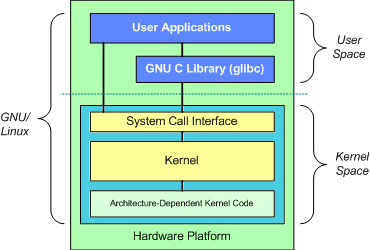
\includegraphics[scale=0.6,clip=true]{figs/Linux_Architecture.png}
  \label{fig:Linux_Architecture}
\end{figure}

\end{frame}

%%%%%%%%%%%%%%%%%%%%%%%%%%%%%%%%%%%%%%%%%%%%%%%%%%%%%%%%%%%%%%%%%%%%%%%

\begin{frame}
\frametitle{The Tanenbaum-Torvalds debate}

\begin{itemize}
\item Very interesting, popular and historical discussion
\item Micro kernel approach represented by Andrew Tanenbaum (Minix)
\item Monolithic approach represented by Linus Torvalds (Linux)

\begin{figure}
  \centering
	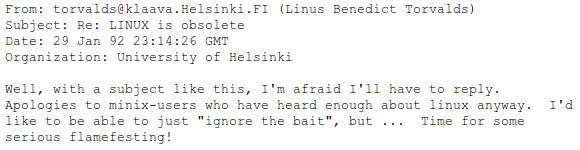
\includegraphics[scale=0.5,clip=true]{figs/Tanenbaum_Linus.png}
  \label{fig:Tanenbaum_Linus}
\end{figure}

\end{itemize}

\begin{center}
{\tiny \url{http://oreilly.com/catalog/opensources/book/appa.html}}
\end{center}

\end{frame}


%%%%%%%%%%%%%%%%%%%%%%%%%%%%%%%%%%%%%%%%%%%%%%%%%%%%%%%%%%%%%%%%%%%%%%%

\section{Kernel Modules}

\subsection{Introduction}

\begin{frame}
\frametitle{What is a kernel module?}

\begin{itemize}
\item Loadable Kernel Module (LKM)
\item The kernel is extended to support other functionalities:
\begin{itemize}
\item Drivers
\item Filesystems
\item Communication Layers
\end{itemize}
\item Flexible approach
\item More efficient memory management
\item No need to recompile or reboot in order to support a new drivers, fs, etc.
\end{itemize}

\end{frame}

%%%%%%%%%%%%%%%%%%%%%%%%%%%%%%%%%%%%%%%%%%%%%%%%%%%%%%%%%%%%%%%%%%%%%%%

\subsection{Kernel module management tools}

\begin{frame}
\frametitle{LKM tools}

\begin{itemize}
\item lsmod
\item insmod
\item rmmod
\item modprobe
\item modinfo
\item depmod
\end{itemize}

\end{frame}


%%%%%%%%%%%%%%%%%%%%%%%%%%%%%%%%%%%%%%%%%%%%%%%%%%%%%%%%%%%%%%%%%%%%%%%

\begin{frame}
\frametitle{LKM tools}

\begin{itemize}

\item lsmod
   \begin{itemize}
   \item List the loaded modules
   \end{itemize}

\item insmod 
   \begin{itemize}
   \item Load the specified module into the running kernel
     \begin{itemize}
     \item \texttt{insmod module\_name} 
     \end{itemize}
   \item Search in the default location of the running kernel
     \begin{itemize}
     \item \texttt{/lib/modules/\$(uname -r)}
     \item Full path to the module can also be provided
     \end{itemize}
   \end{itemize}

\item rmmod 
   \begin{itemize}
   \item Remove the specified module from the running kernel
   \begin{itemize}
     \item \texttt{rmmod module\_name} 
   \end{itemize}
   \item Several modules can be specified at a time
   \end{itemize}

\end{itemize}

\end{frame}

%%%%%%%%%%%%%%%%%%%%%%%%%%%%%%%%%%%%%%%%%%%%%%%%%%%%%%%%%%%%%%%%%%%%%%%

\begin{frame}
\frametitle{LKM tools (II)}

\begin{itemize}

\item modprobe
   \begin{itemize}
   \item Better way to manage the modules (list/load/remove)
   \item Uses the dependency file created by \texttt{depmod}
   \end{itemize}

\item depmod  
   \begin{itemize}
   \item Create a dependency file for LKM
   \item Some modules depend on other modules (symbols)
     \begin{itemize}
     \item A module could need to have other modules loaded first
     \item Eliminate redundancy in the code base
     \end{itemize}
   \item modules.dep file must be regenerated whenever there is a change in the dependencies
   \item In most distros depmod is executed on every boot
   \item All kernel modules must be in the modules.dep file (even the ones with no dependencies)
   \item \texttt{/lib/modules/\$(uname -r)/modules.dep}
   \end{itemize}

\end{itemize}

\end{frame}

%%%%%%%%%%%%%%%%%%%%%%%%%%%%%%%%%%%%%%%%%%%%%%%%%%%%%%%%%%%%%%%%%%%%%%%

\begin{frame}
\frametitle{LKM tools (III)}

\begin{itemize}

\item modinfo
   \begin{itemize}
   \item Provide a list of the module information: author, license, version, dependencies, etc.
   \item \texttt{modinfo module\_name}.

\begin{figure}
  \centering
	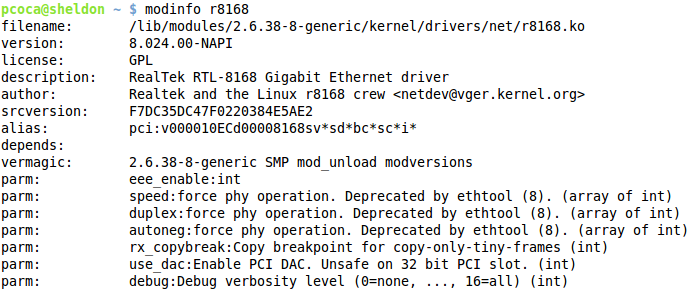
\includegraphics[scale=0.35,clip=true]{figs/modinfo_screenshot.png}
  \label{fig:modinfo_screenshot}
\end{figure}

   \end{itemize}

\end{itemize}

\end{frame}

%%%%%%%%%%%%%%%%%%%%%%%%%%%%%%%%%%%%%%%%%%%%%%%%%%%%%%%%%%%%%%%%%%%%%%%

\begin{frame}
\frametitle{LKM configuration}

\begin{itemize}

\item 2.4 kernel series 
   \begin{itemize}
   \item \texttt{/etc/modules.conf}
   \end{itemize}

\item 2.6 and 3.0 kernel series 
   \begin{itemize}
   \item \texttt{/etc/modprobe.conf}
   \item \texttt{/etc/modprobe.d}
   \item Specify the options loading or removing modules
   \item alias/options/install/remove/include/blacklist
   \end{itemize}

\end{itemize}

\end{frame}

%%%%%%%%%%%%%%%%%%%%%%%%%%%%%%%%%%%%%%%%%%%%%%%%%%%%%%%%%%%%%%%%%%%%%%%
\section{Compiling the kernel}

\begin{frame}
\frametitle{Getting the Linux kernel sources}

\begin{itemize}
\item Download the source file
 
\begin{figure}
  \centering
	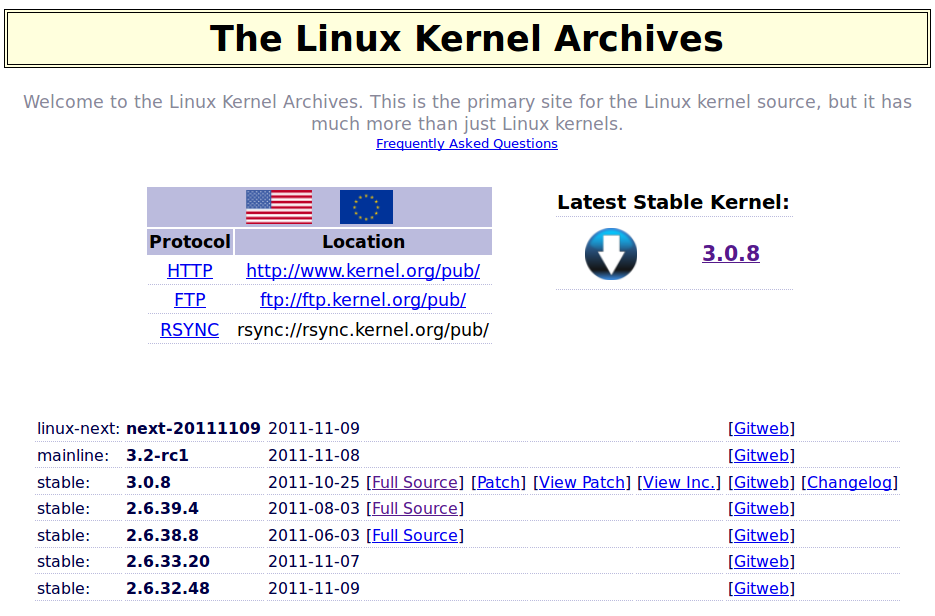
\includegraphics[scale=0.25,clip=true]{figs/kernel_site.png}
  \label{fig:kernel_site}
\end{figure}

\begin{center}
  {\small\url{http://www.kernel.org}}
\end{center}

\end{itemize}

\end{frame}

%%%%%%%%%%%%%%%%%%%%%%%%%%%%%%%%%%%%%%%%%%%%%%%%%%%%%%%%%%%%%%%%%%%%%%%

\begin{frame}
\frametitle{Prepare the system}

\begin{itemize}
\item software/Packages needed 
    \begin{itemize}
    \item gcc compiler
    \item binutils
    \item build-essential
    \item kernel-package
    \item libncurses5-dev (menuconfig)
\end{itemize}
\end{itemize}

\end{frame}


%%%%%%%%%%%%%%%%%%%%%%%%%%%%%%%%%%%%%%%%%%%%%%%%%%%%%%%%%%%%%%%%%%%%%%%

\begin{frame}
\frametitle{Kernel configuration file: .config}

  \begin{itemize}
 	\item Store the kernel configuration
 	\item Configuration files in your /boot directory
           \begin{itemize}
 	   \item \texttt{/boot/config-*}
           \end{itemize}
 	\item We can use one of the config files in /boot as a baseline for our kernel configuration
 \end{itemize}


\end{frame}

%%%%%%%%%%%%%%%%%%%%%%%%%%%%%%%%%%%%%%%%%%%%%%%%%%%%%%%%%%%%%%%%%%%%%%%

\begin{frame}
\frametitle{menuconfig}
 
\begin{figure}
  \centering
	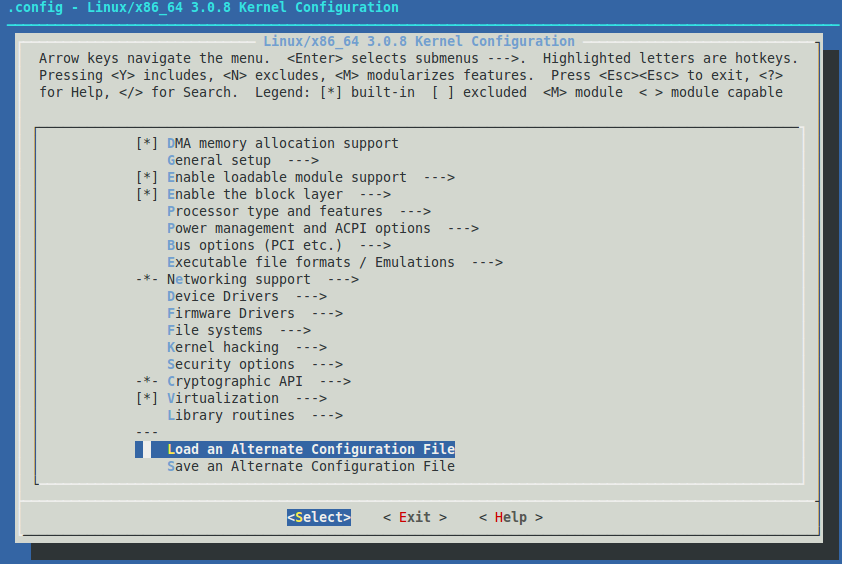
\includegraphics[scale=0.3,clip=true]{figs/menuconfig.png}
  \label{fig:menuconfig}
\end{figure}

\end{frame}


%%%%%%%%%%%%%%%%%%%%%%%%%%%%%%%%%%%%%%%%%%%%%%%%%%%%%%%%%%%%%%%%%%%%%%%

\begin{frame}
\frametitle{menuconfig (II): General setup}
 
\begin{figure}
  \centering
	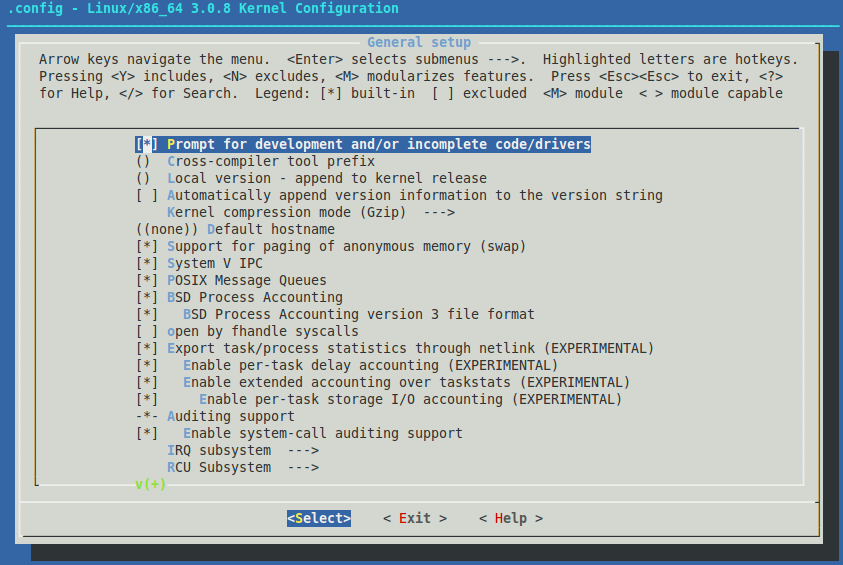
\includegraphics[scale=0.3,clip=true]{figs/menuconfig_generalsetup.png}
  \label{fig:menuconfig_menuconfig}
\end{figure}

\end{frame}

%%%%%%%%%%%%%%%%%%%%%%%%%%%%%%%%%%%%%%%%%%%%%%%%%%%%%%%%%%%%%%%%%%%%%%%

\begin{frame}
\frametitle{menuconfig (III): Example: File systems}
 
\begin{figure}
  \centering
	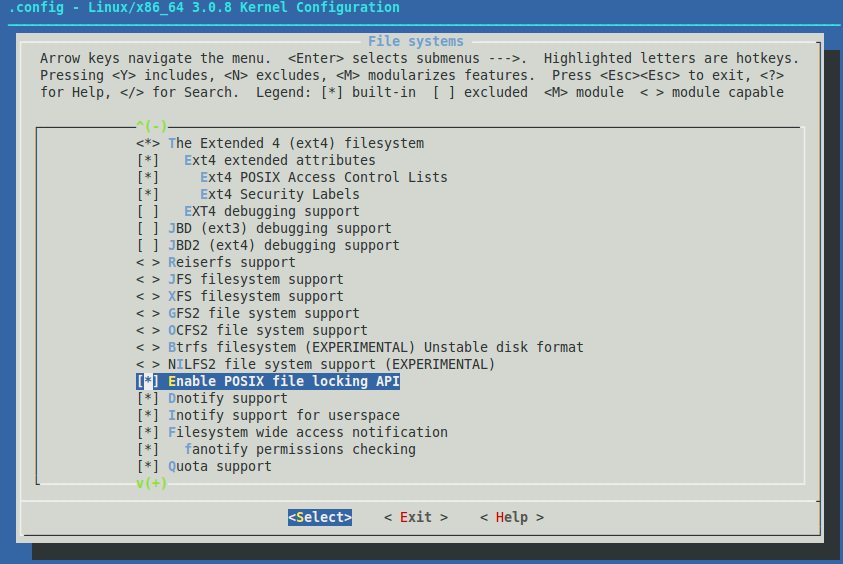
\includegraphics[scale=0.3,clip=true]{figs/menuconfig_filesystems.png}
  \label{fig:menuconfig_filesystems}
\end{figure}

\end{frame}



%%%%%%%%%%%%%%%%%%%%%%%%%%%%%%%%%%%%%%%%%%%%%%%%%%%%%%%%%%%%%%%%%%%%%%%

\begin{frame}
\frametitle{Compilation process}
 
\begin{itemize}
   \item Compile the kernel and modules
      \begin{itemize}
      \item \texttt{sudo make -j8}
      \end{itemize}
   \item Older kernel versions prior to the 2.6 release required the additional step (make modules) to build all needed kernel modules.
   \item Compiling with \texttt{make bzImage} requires to build the kernel modules.
\end{itemize}

\end{frame}

%%%%%%%%%%%%%%%%%%%%%%%%%%%%%%%%%%%%%%%%%%%%%%%%%%%%%%%%%%%%%%%%%%%%%%%

\begin{frame}
\frametitle{Installation process}
 
\begin{itemize}

    \item Install the modules
      \begin{itemize}
      \item \texttt{sudo make modules\_install}
      \item This will place the modules under the proper location
      \item \texttt{/lib/modules/\$(uname -r)}
      \end{itemize}

  \item Install the kernel
      \begin{itemize}
      \item \texttt{sudo make install}
      \item Place several files under /boot/ directory (kernel image, headers, etc)
      \item Any needed initial ramdisk images will be automatically created
      \item Bootloader will be notified (Grub will make a entry in your grub.cfg)
      \end{itemize}
   \item This installation does not overwrite any older kernel images

\end{itemize}

\end{frame}


%%%%%%%%%%%%%%%%%%%%%%%%%%%%%%%%%%%%%%%%%%%%%%%%%%%%%%%%%%%%%%%%%%%%%%%

\begin{frame}
\frametitle{Installation manual steps}

{\small

 \begin{itemize}
     \item \texttt{sudo make modules\_install}
     \item \texttt{sudo cp arch/i386/boot/bzImage /boot/bzImage-3.0.8}
     \item \texttt{sudo cp System.map /boot/System.map-3-0.8}
     \item \texttt{sudo cp System.map /boot/System.map-3-0.8}
     \item \texttt{sudo mkinitramfs -o /boot/init.rd.img-3.0.8 3.0.8}
     \item \texttt{sudo update-grub}
     \item \texttt{sudo grub-install /dev/sda}
 \end{itemize}

}

\end{frame}

%%%%%%%%%%%%%%%%%%%%%%%%%%%%%%%%%%%%%%%%%%%%%%%%%%%%%%%%%%%%%%%%%%%%%%%

\begin{frame}
\frametitle{Initial RAM disk}

 \begin{itemize}
 	\item Initial RAM disk (initrd)
 	\item Temporary file system used in the kernel boot process
 	\item Performs the tasks needed before mounting the root file system
 	\item Part of "stage 2" boot process
 	\item After the initrd kernel modules can be loaded
 	\item Being replaced by the initramfs in the 2.6 series (more flexible and eficient)
 \end{itemize}

\end{frame}


%%%%%%%%%%%%%%%%%%%%%%%%%%%%%%%%%%%%%%%%%%%%%%%%%%%%%%%%%%%%%%%%%%%%%%%

\begin{frame}
\frametitle{Creating an Initial RAM disk image}
 
\begin{itemize}

   \item Device drivers to be loaded in order to mound the root file system
   \item Creation of the RAM disk
      \begin{itemize}
      \item \texttt{sudo mkinitramfs -o /boot/init.rd.img-3.0.8 3.0.8}
      \end{itemize}
   \item Check the bootloader configuration file

\end{itemize}

\end{frame}

%%%%%%%%%%%%%%%%%%%%%%%%%%%%%%%%%%%%%%%%%%%%%%%%%%%%%%%%%%%%%%%%%%%%%%%

\begin{frame}
\frametitle{Creating a Debian Package: make-kpkg}
 
\begin{itemize}
   \item Automate the process and create a debian package with the custom kernel
   \item Execute in the top-level kernel source directory 
      \begin{itemize}
      \item \texttt{sudo make-kpkg --initrd kernel\_image}
      \end{itemize}
   \item The resulting package can be normally installed with dkpg
      \begin{itemize}
      \item \texttt{sudo dpkg -i linux-image-3.0.8-file.deb} 
      \end{itemize}

\end{itemize}

\end{frame}

%%%%%%%%%%%%%%%%%%%%%%%%%%%%%%%%%%%%%%%%%%%%%%%%%%%%%%%%%%%%%%%%%%%%%%%
\section{References}
%%%%%%%%%%%%%%%%%%%%%%%%%%%%%%%%%%%%%%%%%%%%%%%%%%%%%%%%%%%%%%%%%%%%%%%

\begin{frame} 
\frametitle{References}

\begin{itemize}
\item Linux Kernel in a Nutshell. 3rd Edition. (Greg Kroah-Hartman). O'Reilly. December 2006
\item Understanding the Linux Kernel. 3rd Edition. (Daniel P. Bovet, Marco Cesati). O'Reilly. November 2005
\item Linux Kernel Official Website. \url{http://kernel.org}
\item Linux Kernel Newbies. \url{http://kernelnewbies.org}
\end{itemize}

\end{frame}

%%%%%%%%%%%%%%%%%%%%%%%%%%%%%%%%%%%%%%%%%%%%%%%%%%%%%%%%%%%%%%%%%%%%%%%

% Final slide
\usebackgroundtemplate{
\includegraphics[width=\paperwidth]{format/libresoft-bg}}

\frame{
\maketitle
\begin{center}

\includegraphics[width=6cm]{format/gsyc-urjc}
\end{center}
}

\end{document}

